\documentclass[journal]{IEEEtran}
\usepackage{cite}
\usepackage[pdftex]{graphicx}
\usepackage[cmex10]{amsmath}
\usepackage{amssymb}
\interdisplaylinepenalty=2500
\usepackage{array}
\usepackage{dblfloatfix}
\usepackage{caption}
\usepackage{subcaption}

%%%Undefined packages
% \usepackage{todonotes}
% \usepackage{changes}
% \definechangesauthor[name={Min Tan} color=orange]{MT}

\begin{document}
\title{A Time Division Multiplexing Scheme for Area Efficient Digital Low Dropout Regulator Design}
% \title{An Area-Efficient Digital Low Dropout Regulator With Time Division Multiplexing Scheme}
\author{
        Kaixuan~Ye,~\IEEEmembership{Student Member,~IEEE,}
        Min~Tan,~\IEEEmembership{Member,~IEEE,}% <-this % stops a space
\thanks{The authors are with the School of Optical and Electronic Information,
Huazhong University of Science and Technology, Wuhan 430074, China (email:
mtan@hust.edu.cn).}
        }

\markboth{Journal of \LaTeX\ Class Files,~Vol.~14, No.~8, August~2015}%
{K.~Ye\MakeLowercase{\textit{et al.}}: DLDO Paper Draft}


\maketitle

\begin{abstract}
In this paper, we present a novel time division multiplexing (TDM) scheme for the digital low dropout regulator (DLDO) design. By deploying TDM scheme, the proposed TDM DLDO can provide multiple output paths with a single control circuits. To eliminate cross-channel coupling between different output paths, a delay switching technique is proposed. To improve the transient response and save chip area, we also propose a Shared Analog-Assisted (SAA) loop. To demonstrate the working principles of this design, a prototype DLDO of single control circuit dual output paths (SCDO) was fabricated with UMC 130nm 1P8M standard CMOS process. The supply voltage range is 0.6-1.0V, output voltages of two paths are regulated to 0.55-0.95V, and the load current capability of two paths are 80mA and 120mA separately. With few extra control circuits, this SCDO DLDO saves nearly 50\% of the total chip area comparing with two discrete DLDOs. This design can be extended to have multiple outputs and outputs regulated at different voltages. As the control circuit take up more and more area in DLDO, this design points out a very promising method to save the total chip area when multiple LDOs are needed. And the more output paths are regulated, this method should be more area efficient.\\

\begin{IEEEkeywords}
Time division multiplexing (TDM), digital low dropout regulator (DLDO), delay switching, shared analog-assisted loop, area efficient
\end{IEEEkeywords}
\end{abstract}

\section{Introduction}
To obtain a stable and efficient supply, a power management circuit is a fundamental block in many electronic applications\cite{original,coarse-fine,AALDO,AALDO1,NANDbasedAAloop,pipeline,asynchrounous,recursive,AP}. Usually, there are multiple function units in a electronic application, and different function units normally have different requirements for the supply. For example, the supply voltage for analog core circuits is around 1V, while the supply for digital intellectual properties (IP) can be as low as 0.4V. As a result, the power management circuit needs to provide a variety of voltage levels, and this can be realized by employing a hierarchical network which consists of multiple DC-DC converters and low dropout regulators (LDO) pairs, as shown in Fig.\ref{fig:hierarchical}. 

As multiple DC-DC converter and LDO pairs are needed, the chip area for each DC-DC converter and LDO should be small. To save the DC-DC converter chip area, a single inductor multiple outputs (SIMO) DC-DC converter is proposed in \cite{SIMODCDC,SIMODCDC1,SIMODCDC2}. Traditionally, an off-chip inductor is required for every DC-DC converter, however, this not only increases the number of required on-chip pads, but also bring about great noise to the circuits. In SIMO DC-DC converter, the inductor is shared by multiple different sub-converters, and Fig.\ref{fig:DCDC} shows the diagram of a SIMO DC-DC converter. Different sub-converters are connected to the inductor at different moment, so each sub-converter can realize its function at its corresponding period. As long as the switching frequency is fast enough, all sub-converters can be regarded as working continually. So the SIMO DC-DC converter can fulfill the function of multiple DC-DC converters and the chip area for DC-DC converters can be greatly reduced.

\begin{figure}[t!]
    \centering
    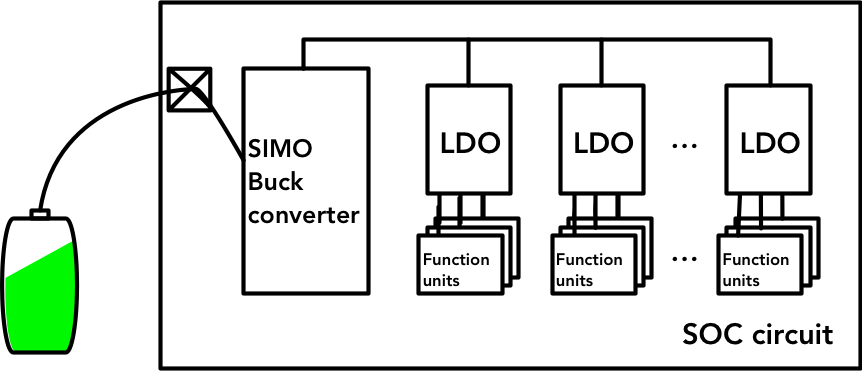
\includegraphics{pic/DLDOsche/SOCcircuit.pdf}
    \caption{Hierarchical power managing network}
    \label{fig:hierarchical}
\end{figure}
As for the LDOs, they are traditionally analog circuits constructed with an error amplifier, a buffer driver and a power stage\cite{ALDO1,ALDO2,ALDO3,ALDO4,ALDO5}. The current of power stage is controlled by the size and gate to source voltage of the power transistor. Since minimum headroom voltage must be maintained for the error amplifier and buffer driver to make sure they can operate in saturate region, the gate to source voltage for power transistor is relatively small in most cases. Consequently, the size of power transistor should be increased to meet the load current requirement. Consider a typical analog LDO in which the load current capability is 100mA, the power stage area can be as large as $\rm 0.088 mm^2$, taking up more than 70\% of the whole chip area\cite{ALDO5}. To save the power stage area, digital LDO (DLDO) was first proposed in \cite{original}. Contrary to the analog counterpart in which the output current is controlled by the gate to source voltage of power transistor, the output current of DLDO is controlled by the number of turned-on units of the power PMOS array. Since each unit can be fully turned on, the size of power stage can be significantly reduced under the same supply voltage and load current requirements\cite{AP}.

\begin{figure}[t!]
    \centering
    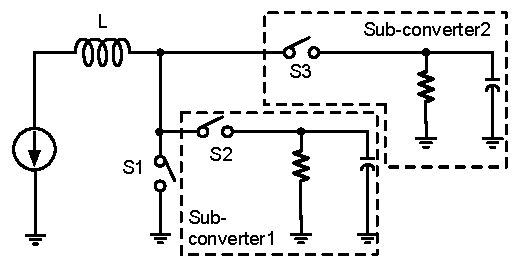
\includegraphics[width=\linewidth]{pic/TDM/DCDC.pdf}
    \caption{SIMO DC-DC converter}
    \label{fig:DCDC}
\end{figure}
Nevertheless, the original DLDO suffer from large dropout and ripples, and many advanced techniques have been proposed to tackle these problems. In\cite{coarse-fine}, a coarse-fine switching technique was proposed to alleviate the ripple problem. It employs two power PMOS arrays with units of different sizes. When load change happens, the power PMOS array with units of large size is connected to loop, so the output can recover to the regulated voltage fast. And when DLDO reaches steady state, the smaller power PMOS array is connected to the loop, hence turning ON/OFF each unit give rise to little ripple to the output.  In \cite{AALDO,AALDO1,NANDbasedAAloop}, in order to improve the transient response, an analog-assisted (AA) loop consisting of coupling capacitor and resistor is added. The AA loop can sense the output undershoot and feed it back to the driver of power PMOS array, therefore the power PMOS array can response to the output before the clock rising edge, consequently, the undershoot of DLDO is significantly reduced. In \cite{pipeline}, it adopts a pipeline control structure and a 3-D power stage to realize the multi-step switching scheme. As a result it speeds up the transient response while maintaining a small output voltage ripple. And in \cite{recursive}, it proposed a recursive DLDO which improves the performances by applying a SAR-like binary search algorithm and a sub-LSB pulse width modulation duty control scheme. 

Although all above techniques can be effective in some way, the control circuit which is very small in analog LDO takes up more and more chip area when the control method becomes complicated. In some cases, the control circuit area can be equivalent even greater than the power stage area, and this undoubtedly neutralizes the area-efficient benefit of a smaller power stage. To get a smaller power stage as well as a smaller control circuit, \cite{ClassDLDO} propose a LDO driven by a class-D controller. The class-D LDO consists of an error amplifier, a class-D controller and a power stage. The error amplifier amplifies the error voltage between feedback voltage and reference, and the class-D controller converts it to a pulse width modulation (PWM) signal which drives the power stage. As the class-D controller can have rail-to-rail output range, the output current density of the power transistor is significantly increased comparing with the traditional analog LDO. However, a bulky output capacitor as large as 1$\rm \mu F$ is needed in this structure, which is not suitable for IC implementations.

In this paper, we propose a novel time-division-multiplexing (TDM) scheme to realize a area efficient DLDO design. And the remainder of this paper is organized as follow. In section II, we discuss the necessity and difficulties to apply TDM scheme to DLDO design. In section III, we present the architecture and working principles of the proposed TDM DLDO design. In section IV, we interpret the circuit implementation and design considerations. In section V, we show the measurement results along with comparisons. And in section VI, we conclude our proposed design.

% So it becomes a very interesting topic how we can improve the area efficiency of the control circuit. To improve chip area efficiency, the time-division-multiplexing (TDM) scheme has been applied in many other circuits and has achieved great success. As is a digital concept, this scheme should be available to the DLDO design as well.
%%This paragragh needs further tuning.
\section{Discussions on TDM DLDO}
TDM is a method originally used in signal transmissions. In TDM scheme, signals are interleaved with others and each signal occupy the signal path only a fraction of time in an alternating pattern. In the early days of electrical communication when signal must be transmitted with a medium such as copper wire, this method significantly saved the cost and equipment\cite{TDM}. Motivated by the great success of TDM scheme in signal transmissions, it also finds many applications in circuit designs, and the SIMO DC-DC converter mentioned above is classic example. In SIMO DC-DC converter, the connection of different sub-converters are controlled by switches. By adopting a specific switch control signal, different sub-converters are connected to the inductor alternately, hence the inductor is working in TDM scheme. Another example is the silicon Micro Ring Modulator (MRM). The MRM is believed to be the most important device to realize optical interconnect, which have been proposed to displace electrical interconnects as the next generation I/O links due to its ultra-wide bandwidth and low loss advantages \cite{wangzhicheng}. In MRM, it usually requires a feedback control circuit to stabilize the resonant wavelength of micro ring, and the control circuit is much larger than the micro ring itself. So \cite{wangzhicheng} applies the TDM scheme to the control circuit, and it significantly saves the total chip area.

\begin{figure}[t!]
    \centering
    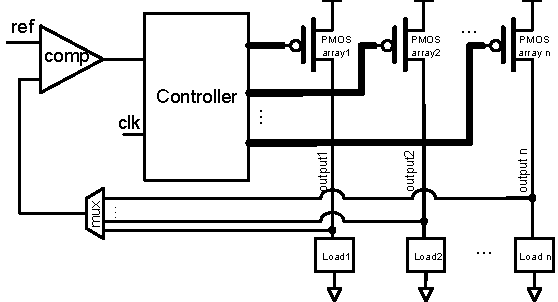
\includegraphics[width=\linewidth]{pic/TDM/TDMDLDO.pdf}
    \caption{the proposed TDM DLDO}
    \label{fig:TDMDLDO}
\end{figure}
As the control circuit of DLDO is increasingly large, we can also apply the TDM scheme to DLDO controller to maintain the area-efficient benefit of DLDO. Fig.\ref{fig:TDMDLDO} shows the diagram of the proposed TDM DLDO, the main idea is very straightforward, outputMux select different output paths to the comparator for a fraction of time in an alternating pattern. In the corresponding time fraction of each path, the comparator compares the output voltages with the reference, and the comparison result serves as the input signal of the controller, which finally determines the states of the power PMOS array. As multiple outputs share the common control circuit at different time fractions, the proposed DLDO is operating in TDM scheme. Although the TDM DLDO concept is straightforward, two main technical difficulties exists before we can implement it in reality.
\subsection{Cross channel coupling}
In electronic applications when multiple supply voltage levels are required, the current or voltage variation at one supply should not affect others. This requirement can be easily satisfied when multiple DLDOs are employed, however, in TDM DLDO, how to avoid the cross channel coupling between different paths is the foremost challenge. Fig.\ref{fig:shift} shows parts of the shift register structure which serves as the controller in most DLDO design. The $compOut$ determines which signal is connected with the input of D-type flip flop (DFF), and DFF transfers the input to the next stage at every rising edge of $clk$. In other word, the shift register maintains the states of all units of power PMOS array for half $clk$ period. In TDM DLDO, the load current at different output paths differs each other, so the units of power PMOS array should have different states. However, when different output paths switch, the shift register which maintains the states of previous path is directly  connected with the power PMOS array of the next path. If the load current at these two paths vary significantly, a large cross channel coupling will occur at the next output path. 

Another factor that would lead to cross channel coupling comes from the comparator. In most DLDO design, the comparator is a sense amplifier based structure,and this kind of structure can only compare at half period and would latch the result at another half period. Hence, if the path switch happens at the half period when comparator latch the result, the $compOut$ signal would not change no matter what are connected with the comparator input terminals. If the relationship between output voltage and reference differs at different path, this would also cause cross channel coupling at the output.

\begin{figure}[t!]
    \centering
    \includegraphics[width=\linewidth]{pic/struc/shiftRegister.pdf}
    \caption{Parts of shift register in DLDO}
    \label{fig:shift}
\end{figure}
\subsection{Maintain power PMOS array states}
Another technical difficulty to realize TDM DLDO is how to maintain the PMOS array states at off-loop path. In SIMO DC-DC converter, the current running through inductor charges the capacitor, so the output voltage can be maintained even if the sub-converter is off the control loop. But in TDM DLDO, the output voltage is maintained by the proper states of power PMOS array. And if the power PMOS array of one path is off the control loop, the state of each unit will be severely disturbed by the large parasite gate to drain capacitor.

\section{Architecture and working principle of the proposed TDM DLDO}
\subsection{Architecture}
From above discussions, we can conclude that apply TDM scheme to controller is effective to keep the area-efficient benefit of DLDO, but we need to propose a structure that can solve the cross channel coupling as well as maintain the power PMOS array states of off-loop paths first. Fig.\ref{fig:diag} shows the architecture of our proposed TDM DLDO. To simplify the design process, we only demonstrate the situation when the common controller is share by two output path. And the proposed architecture mainly consists of a comparator, a outputMux, two groups of latches and two power PMOS arrays. To alleviate the output ripple, we adopt units of two different sizes in each array, and these two kinds of units are driven by two separate shift registers. To tackle the cross channel coupling, all bits of the shift registers can be set/reset. And the two groups of latches are introduced to maintain the power PMOS array states of the off-loop path. In addition, we also employ a shared analog-assisted (SAA) loop to improve the transient response.

\begin{table}[t!]
\centering
\caption{Comparison of TDM DLDO and discrete DLDOs}
\label{tab:compare}
\renewcommand{\arraystretch}{1.8}
\begin{tabular}{|c|c|c|}
\hline
 & n paths TDM DLDO & n discrete DLDOs \\ \hline
Power PMOS arrays & n & n\\\hline
Comparators & 1 & n \\\hline
Shift registers & 2 & 2n \\\hline
AA loop & 1 &n\\\hline
Latch groups & n & n\\\hline
MUX & n+1 & 0\\\hline
Asyn. set/reset cir. & 1 &0\\\hline
\end{tabular} 
\end{table}
Table \ref{tab:compare} compares the structure of n paths TDM DLDO and n discrete DLDOs. In TDM DLDO, the comparator, shift register and AA loop are shared by all paths, while all of them should be separately assigned to each other in n discrete DLDOs. The latch groups in TDM DLDO are employed to maintain the power PMOS array states, while it can also serves as the buffer stage which plays a major role in AA loop technique\cite{AALDO,AALDO1,NANDbasedAAloop}. Hence, all the extra overhead for TDM DLDO is an asynchronous set/reset circuit and n+1 multiplexers. As comparator, shift register and the AA loop consists the main part of DLDO controller while the asynchronous set/reset circuit and multiplexer only takes up negligible chip area, this TDM scheme undoubtedly saves the chip area of DLDO significantly.

\begin{figure*}[t!]
    \centering
    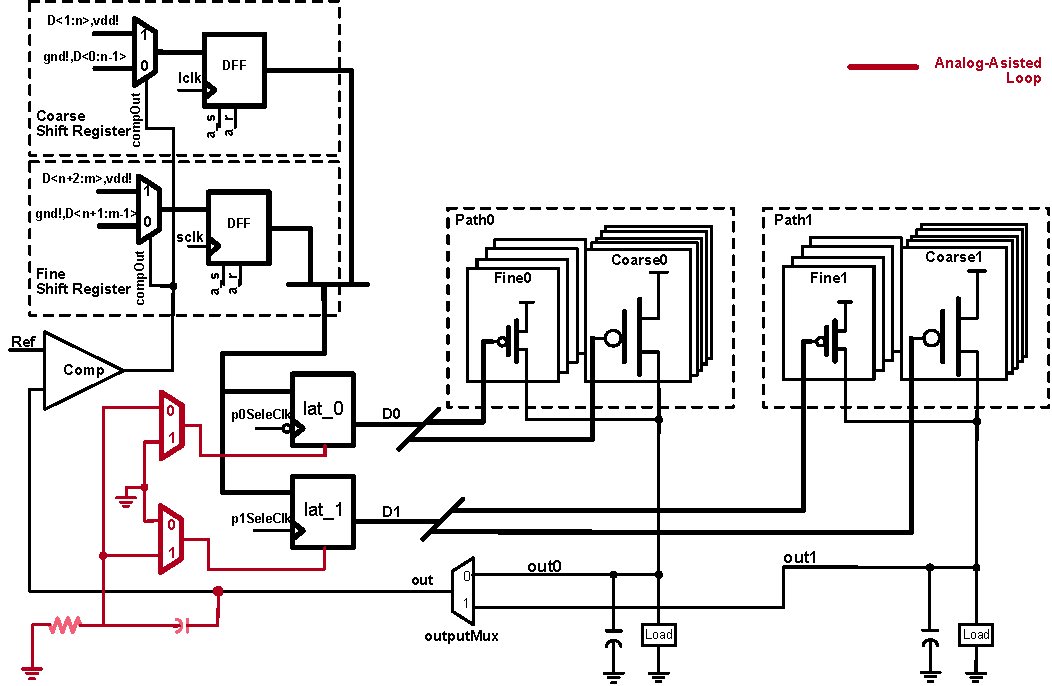
\includegraphics{pic/struc/sche.pdf}
    \caption{Structure of the proposed TDM DLDO}
    \label{fig:diag}
\end{figure*}
\subsection{Delay switching technique}
\begin{figure}[t!]
    \centering
    \includegraphics[width=\linewidth]{pic/struc/AsynSet.pdf}
    \caption{Asynchronous set/reset circuits}
    \label{fig:Asyn}
\end{figure}
As we mentioned before, cross channel coupling is one of the main interference in TDM DLDO. And cross channel coupling occurs because the shift register maintains the states of previous path when it should connect with the power PMOS array of the next path at the path switching instance. To tackle this problem, we can pre-load the power PMOS array states of next path to shift register before PMOS array and shift register are connected together. And that is main idea of the proposed delay switching technique.

Fig.\ref{fig:timing} shows the timing diagram of the proposed TDM DLDO. We denote $clk$ as the system clock which drives comparators and shift registers, and $path$ is the output paths selection signal that determines which output path is to be connected with the DLDO control circuit, when multiple output paths share the DLDO controller, there needs to be several $path$ signals, however, we only need one $path$ signal to distinguish the two output paths in our demonstration circuit. $sele$ is a pulse signal which arises at both rising and falling edges of the $path$ signal. The duration of $sele$ pulse is the time window for the asynchronous set/reset circuit to work. $p0SeleClk$ and $p1SeleClk$ derive from the logic combination of $path$ and $sele$, and this two derivative signals control the working conditions of two latch groups. Note that $lat\_0$ is low active while $lat\_1$ is high active. $D0$ and $D1$ denote the working conditions of the two output paths, the yellow period denotes that the power PMOS array states are latched, the orange period denotes that the asynchronous set/reset circuit is loading the power PMOS array states of the next path to the shift register, and the dashed period denotes the actual working period of each path. At last, $D$ reveals the address of the states maintained in the common shift register.

\begin{figure}[t!]
    \centering
    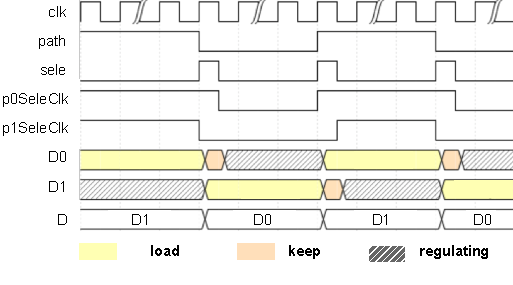
\includegraphics[width=\linewidth]{pic/struc/timing.pdf}
    \caption{Timing diagram of the proposed design}
    \label{fig:timing}
\end{figure}
\begin{figure}[t!]
    \centering
    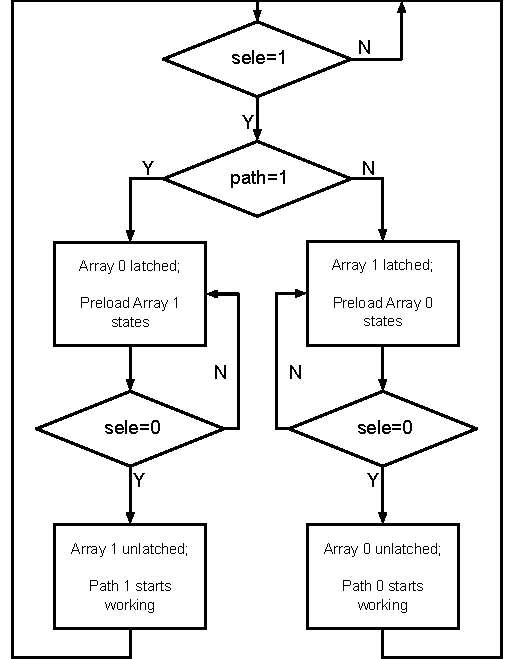
\includegraphics[width=\linewidth]{pic/struc/flowChart.pdf}
    \caption{Flowchart of the delay switching technique}
    \label{fig:flowchart}
\end{figure}
Fig.\ref{fig:flowchart} is the flowchart that illustrates the operating process of the delay switching technique. At every switching instance of $path$, a $sele$ pulse arise and $sele=1$ is set up. Then the DLDO control circuit checks which path is to be connected, and in our demonstration circuit, $path=1$ denotes output path 1 is to be connected while $path=0$ denotes output path 0 is to be connected. For example, when $path=1$, then the TDM DLDO control circuit is to be connected with output path 1, and the power PMOS array at path 0 is disconnected with the control circuit and latched immediately. At that time, the power PMOS array 1 is not connected yet, so they are latched by the latch group as well. However, $sele=1$ set up a time window for the asynchronous set/reset circuit, and they pre-load the states of power PMOS array 1 to the shift register at that time. When the $sele$ pulse disappears, the asynchronous set/reset circuit stops working and the shift register is ready to be connected with power PMOS array 1. Hence array 1 is unlatched, and the DLDO control circuit and power PMOS array are finally connected after a $sele=1$ delay. Then path 1 starts to regulate output like a normal DLDO until the path switching happens again. As the states of previous path maintained in shift register are replaced with its own states before the power POMS array is to be connected, the cross channel coupling can be completely eliminated in theory.

The structure of asynchronous set/reset circuit is shown Fig.\ref{fig:Asyn}. It is comprised of n units, and each unit control a single bit of the shift register. In each unit, there are a multiplexer, a inverter and two AND gate. The multiplexer is controlled by the $path$ signal and it transfers the power PMOS array state to the input of two AND gate. When $sele=1$, the two AND gates are enabled and the unit asynchronously set/reset the corresponding bits of the shift register immediately. As the power PMOS array states of the inactive path is latched by the latch group, the state maintaining problem of TDM DLDO design is solved with the delay switching technique as well.
\subsection{The shared analog-assisted loop}
\begin{figure}[t!]
    \centering
    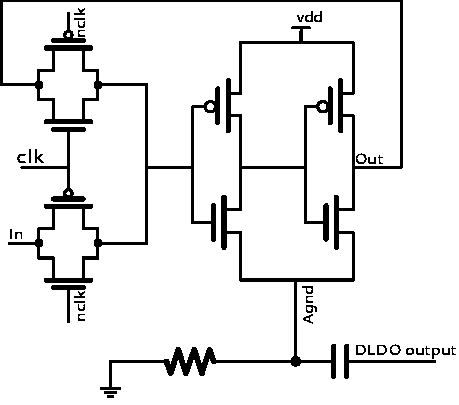
\includegraphics[width=\linewidth]{pic/struc/latch.pdf}
    \caption{The latch structure in TDM DLDO}
    \label{fig:lat}
\end{figure}
\begin{figure}[t!]
    \centering
    \includegraphics[width=\linewidth]{pic/struc/sharedAAloop.pdf}
    \caption{The shared AA loop in TDM DLDO (a)When Path 0 is active (b)When Path 1 is active}
    \label{fig:sharedAAloop}
\end{figure}
One of the most severe drawbacks of DLDO is the poor transient response. For example, when load current changes from light to heavy, an undershoot would appear at the output because the power stage could not provide enough current to the load. In analog LDO, this undershoot would feedback to the error amplifier, then the error amplifier output alter the gate voltage of the power transistor immediately. The response time is limited by the bandwidth of LDO, and is usually very short. However, the DLDO can not response to the output undershoot immediately. As the shift register can only refresh its states at every clock rising edge, the power PMOS array states would not change until the clock arriving no matter how large the undershoot is. This problem could be partly solved if we adopt a faster system clock, however, this would lead to more power consumption. In \cite{AALDO,AALDO1,NANDbasedAAloop}, an analog-assisted loop was proposed. It consists of a resistor and a capacitor, and these two devices forms a high-pass network. At steady state, the output voltage is a relatively stable value and the AA loop does not take effect. And when load current change happens, this AA loop can sense the undershoot at output immediately, then it transfer this signal to the latches of the power PMOS array. as shown in Fig.\ref{fig:lat}, this would bring an undershoot at the $Agnd$ node and gate voltage of the PMOS array would drop down as well.  Therefore, the power PMOS array could provide more current to the load even before the clock signal arrives.

The AA loop significantly improves the transient response of DLDO, however, the on-chip capacitor and resistor takes up great chip area. As we mentioned before, the AA loop actually only takes effect when load change, and stay idle at most time. Hence, it has the potential to be shared by different paths in TDM scheme. And Fig.\ref{fig:sharedAAloop} shows our proposed shared AA loop structure. Apart from the capacitor and resistor, the only extra overhead to realize shared AA loop is $n$ multiplexers. In our demonstration circuit, $n=2$, and the two input terminals of all multiplexers are connected with GROUND and the $V_{SSB}$ node of the shared AA loop separately. When path 0 is active, the $V_{SSB}$ of shared AA loop is connected with the $Agnd$ of $lat\_0$, and the $Agnd$ of $lat\_1$ is connected with the GROUND. Hence, the shared AA loop helps improving the transient response of path 0, and the states of path 1 power PMOS array are latched. Similar condition happens as well when path 1 is active.
\subsection{Coarse-fine switching}
\begin{figure}[t!]
    \centering
    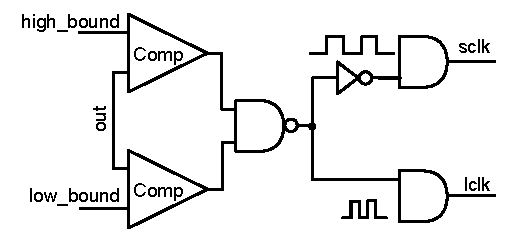
\includegraphics[width=\linewidth]{pic/struc/peak.pdf}
    \caption{Coarse-fine switching controller}
    \label{fig:coarse-fine}
\end{figure}
Coarse-fine switching technique is another method to improves the DLDO performance. In the original DLDO\cite{original}, all the units in power PMOS array are equal-sized. If the units are too small, turning ON one unit can only provide very small current to the load and have little influence on the output voltage. When load current changes, the recovery time could be intolerably large. In addition, the current capability of the DLDO is limited as well. However, if the units are too large, the recovery time can be reduced, but every single unit would bring about large current and voltage variation at the output, so the accuracy of DLDO is degraded. In summary, there is a trade-off between accuracy and speed. To break through this trade-off, the coarse-fine switching technique was proposed in \cite{coarse-fine}. It adopts a power PMOS array with units of different sizes. And each kind of unit is driven by a separate shift register. At steady state, the fine shift register toggles units of smaller size, so it would bring about little influence on the output voltage. And at the load changing state, fine shift register is disabled, and the coarse shift register drives the larger units in power PMOS array to achieve a relatively short recovery time. The switching between coarse and fine shift register is controlled by the coarse-fine switching controller as shown in Fig.\ref{fig:coarse-fine}. The controller compares the output with two boundaries, and the comparison result is processed by a NAND gate. If the output is within two boundaries, the controller enables the upper AND gate, and clock signal transfers to $sclk$ while the $lclk$ is zero. Otherwise, the clock signal transfers to $lclk$ and $sclk$ is zero. The $lclk$ and $sclk$ drives coarse and fine shift registers separately. And the combination of these two shift registers achieves short recovery time as well as accurate output.

\section{Circuit implementation and considerations}
\subsection{Maximum output paths}
In TDM DLDO, one of the most important parameter is the maximum number of output paths. Considering the easiest condition when the load changes at a regular frequency, and we denote the load changing period as $T_{load}$. Assuming that load change happens exactly after TDM DLDO finishes the path switching process and operates like a normal DLDO. Denoting the response time of the DLDO is $T_{res}$ and the duration of $sele$ pulse is $T_{sele}$. The response of the proposed TDM DLDO when load change happens is shown in Fig.\ref{fig:sele}, $output$ is the confluent output voltage of all paths, and the gray, yellow and pink fraction denote the voltage variation at corresponding paths, and $load_0$ to $load_n$ denote the load changing conditions of different paths. Also note that the $sele$ signal is the time window for the asynchronous set/reset circuit, as we assume load change happens exactly after TDM finish the path switching process, the pulses at $sele$ disappear right before the load changes. From Fig.\ref{fig:sele} we can easily conclude that the maximum number of regulated output paths is:
\begin{equation}
 N \leqslant \frac{T_{load}}{2\times(T_{sele}+T_{res})}
\end{equation}

The response time of each path is determined by the swing of load change, the size of unit in power PMOS array and the clock frequency. According to (1), the shorter the response time is, the more output paths the TDM DLDO could handle. Generally speaking, a shorter response time can be achieved by adopting faster clock or larger power PMOS array units.

\begin{figure}[t!]
    \centering
    \includegraphics[width=0.9\linewidth]{pic/consid/sele.pdf}
    \caption{The response of TDM DLDO when load changes}
    \label{fig:sele}
\end{figure}
The duration of $sele$ is determined by the response time of the asynchronous set/reset circuit and shift register. Since $T_{sele}$ serves as a time window, if $T_{sele}$ is too short, the asynchronous set/reset circuit may be not ready to load its input to the shift register, so the delay switching technique fails and great cross channel coupling between different paths may happen. However, on the other hand, $T_{sele}$ should not be too long either. In delay switching technique, all paths are disconnected with the DLDO control circuit during the $T_{sele}$ period and could not response to the load changing at that time. So if $T_{sele}$ is too long, there is a risk that if load change happens during that period the undershoot/overshoot at the output may grows out of control. In addition, according to (1), a longer $T_{sele}$ also limits the maximum number of regulated output path the TDM DLDO can handle. In our design, we set $T_{sele}$ to be half the clock period, and it can fulfill its function properly.

Normally the load change frequency is not high in many electronic applications, for example, the Internet of Thing (IoT) applications. Hence, the maximum number of output paths the proposed TDM DLDO can handle is on the order of tens. However, if more paths are arranged in the TDM DLDO, the allocated regulating period for each path decreases, and risk grows that load change may happens during the disconnected period at one path. And this would lead to the output voltage variation grows out of control. Therefore we should arrange the actual number of output paths according to application scenarios.

Note that when the output reaches the nearby of the reference, either turning on or off one PMOS array unit may change the comparison result and limit cycle oscillation (LCO) occurs. In other word, the DLDO only regulate the output at the switching status, and disconnect the PMOS array from the shift register at the stable status may even be beneficial to the performance. 

\subsection{``sele'' signal duration}
The ``sele'' signal in  our design has two functions. Firstly, it can modulate the ``path'' signal and generates ``p0SeleClk'' and ``p1SeleClk'' which control the active period of the two paths. In some way, this signal serves as a guard period between the two processing periods, so the duration time of ``sele'' needs to be long enough to avoid cross-talk between two paths. Secondly, ``sele'' is the enabled signal of the asynchronous set/reset circuit which load the states of the next path to the shift register before it is connected to the loop. So the duration of ``sele'' needs to be longer than the response time of shift register. However, from another perspective, the ``sele'' signal duration should not be too long as well. During the active period of the``sele'' signal, both paths are not connected to the control loop of the DLDO. On the one hand, this decreases efficiency of the circuit, on the other hand, there is risk that load change may happens during the ``sele'' period, so large undershoot may appear if the path is not connected to the loop. In our design the pulse duration of ``sele'' signal is about half period of the clock signal. 
\subsection{``path'' signal duration}
``path'' signal determines which path is to be connected to the control loop. We only demonstrate the two paths case in this paper, so only one ``path'' signal is needed, in which HIGH select one path, and the LOW selects the other one. If $n$ ``path'' signals are provided, the maximum numbers of paths that the TDM DLDO can regulate is $2^n$. There are two mainly perspectives to choose the ``path'' signal period. First, we can determine it by the load change frequency. if load change drastically at one path, it needs to be connected to the controlled loop for longer time, otherwise large undershoot or overshoot may occurs. But if the load changes not so frequently at one path, we can just latch the PMOS array states and connect the control circuit to other paths to improve the efficiency of control circuit. However, in this scheme, we need to know how the load changes on each paths in advance. Another way is to  simply increase the ``path'' signal frequency to avoid the large undershoot and overshoot situations. If the ``path'' signal is fast enough, all paths can be regarded as connected to the control loop simultaneously, and the undershoot or overshoot is similar to the one path situation. Nevertheless, assuming the regulating period for all paths is $T$, and the response time of each path is $T_{res}$, then:
\begin{align}
\rm \frac { T}{2^n} &> T_{res}\\
\rm T &> 2^nT_{res}
\end{align} 
\subsection{R and C selection in shared AA loop}
The high-pass network constructed by the resistor and coupling capacitor in the AA loop sense the undershoot and overshoot at output and transfer it to the gate of PMOS array units, so the path can response to load change asynchronously. The effect of the AA loop is determined by the time constant of the high-pass network. Generally, a large time constant helps the output to recover to the regulated voltage faster. As capacitor takes up much larger area in the layout, we usually choose a relatively large resistor to increase the time constant value. However, different from the design in \cite{NANDbasedAAloop,AALDO1}, we need to share the AA loop between different paths. As a result, if the time constant is too large, the voltage at $V_{SSB}$ may not return to GROUND yet when the path switching happens, and it would cause the PMOS array at another path response to this change. In other word, cross-channel coupling happens between different paths. So there is a trade off between cross-channel coupling and response time.
\subsection{Sense amplifier based comparator and D-type flip flop}
Comparator and D-type flip flop are two core circuits in the DLDO design. Comparators are usually sense amplifier based dynamic comparator. The schematic that adopted in our paper is shown in Fig.\ref{fig:comp}\cite{comparator}. It has two stages, the pre-amplify stage consisting of M8 - M12, and the regenerate stage which is constructed by M1 - M7. When `$clk$' is low, M1 and M12 turn off and M8 and M9 turn on, the supply charge the gate of M4 and M7 through M8 and M9. As both M4 and M7 turn on, ``out+'' and ``out-'' are dropped to GROUND and turn on M2 and M3. When `$clk$' becomes high, M1 turns on, so the supply charge the ``out+'' and ``out-'' nodes initially. As M12 turns on the pre-amplify stage, the difference at M10 and M11 is amplified. The outputs of pre-amplify stage controls the charge speed of ``out+'' and ``out-''. Once one of the nodes first reaches the threshold voltage, the regenerate stage forms a positive feedback, and this node become HIGH and the other one becomes LOW.

D-type flip flop is another structure which plays an important role in the DLDO design, but hardly mentioned in the literature. The D-type flip flop adopted in our design is also a sense amplifier based structure as shown in Fig.\ref{fig:DFF}, and the working principle of it is similar to the dynamic comparator.  When clock signal is low, M10 is closed,so the sense amplifier stop working, and M1 and M4 charge the nS and nR to high, as a result, the output latch keep the previous input data. When clock signal becomes high, M1 and M4 are closed, and M10 is open, the sense amplifier acts like a positive feedback network, input D and nD transfer the data to the output of the sense amplifier, and the latch keep the result until next clock falling edge arrives. The structure transfer data only at the clock edge, so it works like a D-type flip flop.
\begin{figure}[t!]
    \centering
    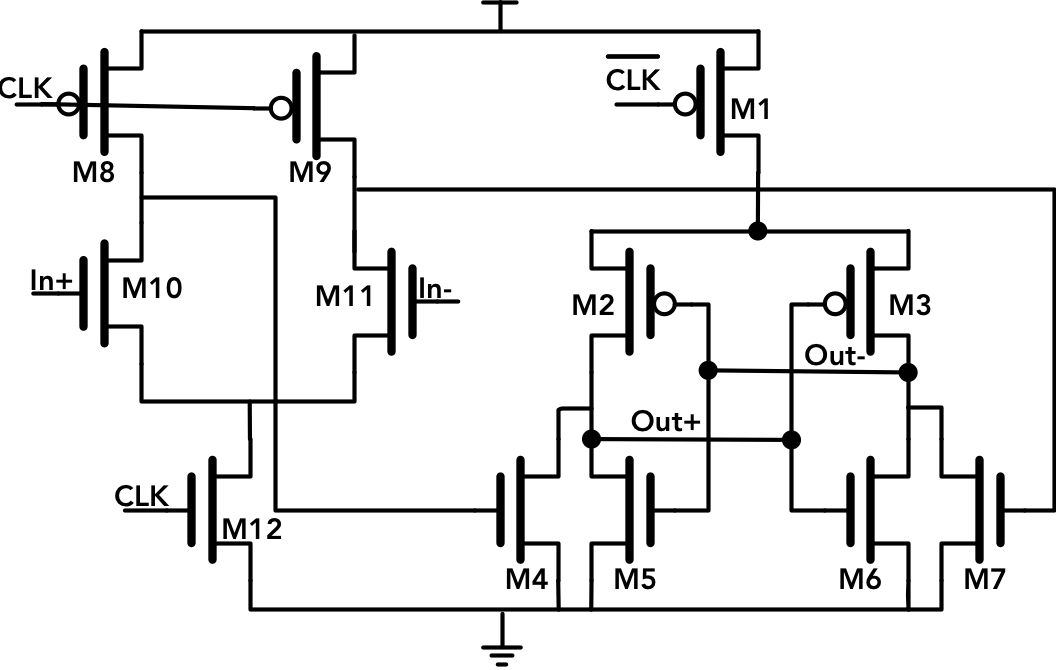
\includegraphics[width=0.9\linewidth]{pic/struc/comp.pdf}
    \caption{Schematic of sense amplifier based dynamic comparator}
    \label{fig:comp}
\end{figure}
\begin{figure}[t!]
    \centering
    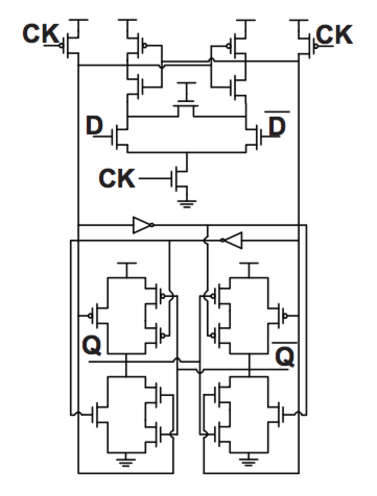
\includegraphics[width=\linewidth]{pic/struc/DFF.pdf}
    \caption{Schematic of sense amplifier based flip flop}
    \label{fig:DFF}
\end{figure}

\section{Measurement results and comparison}
\begin{figure}[t!]
    \centering
    \includegraphics[width=0.9\linewidth]{pic/resu/layout.pdf}
    \caption{The layout of the TDM DLDO}
    \label{fig:layout}
\end{figure}
\begin{figure}[t!]
    \centering
    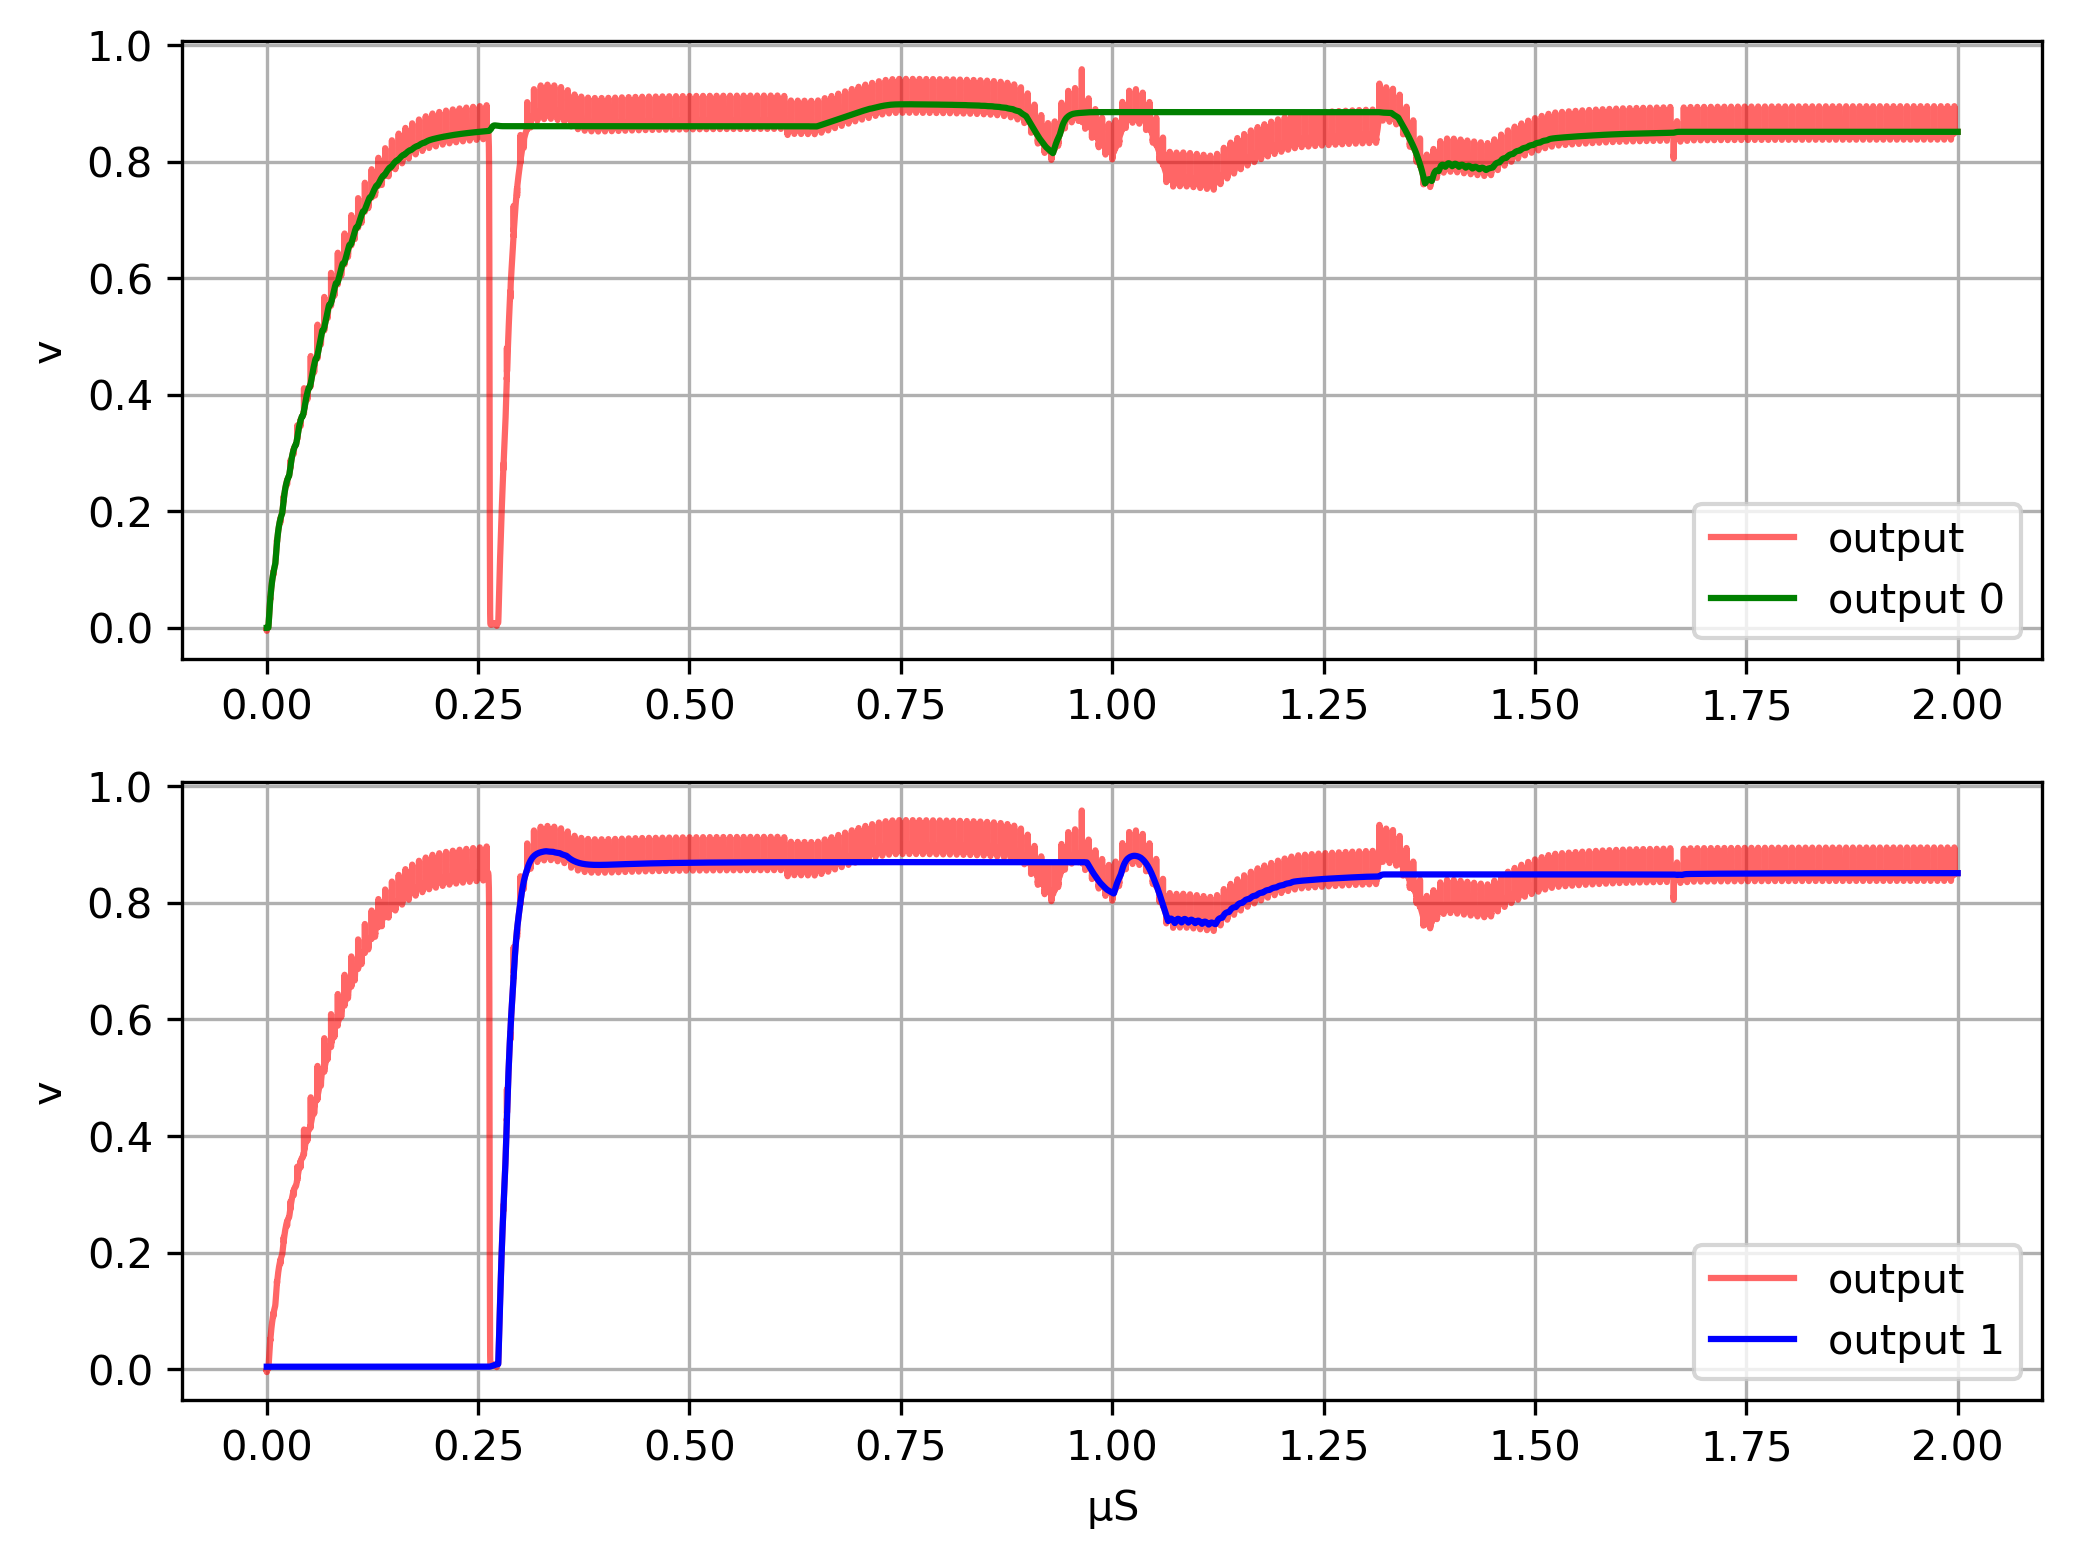
\includegraphics[width=\linewidth]{pic/resu/output.pdf}
    \caption{Output voltage of the proposed TDM DLDO}
    \label{fig:output}
\end{figure}
The TDM DLDO was fabricated in UMC 130 nm 1P8M CMOS process. The layout of the proposed design was shown in Fig.\ref{fig:layout}. The area of the core circuit is about 0.1855$\rm mm^2$. as shown in Fig.\ref{fig:layout}, the shift register and control circuit takes up much more area than power PMOS array. As we can share the shift register almost at no cost, the total chip area of TDM DLDO is greatly reduced when comparing with two DLDOs. Fig.\ref{fig:output} shows the output voltages of the proposed TDM DLDO. The red line stands for confluent output of the two paths, and output 0 and output 1 are the output voltages at two paths respectively. It is clearly shown that the output 0 and output 1 coincides with the output line at different time period and no cross-channel coupling exists at the switching instance. The largest undershoot at both paths is about 200 mV. Fig.\ref{fig:curr} shows the load current changes at two paths. Load change happens when their corresponding path is connected with the control circuit. The edge time of the load change is about 120 ns, and load change from 2 mA to 80 mA at path 0 and from 2 mA to 90 mA at path 1. Fig.\ref{fig:gnd} shows the $V_{SSB}$ and analog ground voltage of the latch groups. The red line stands for the $V_{SSB}$ voltage of the shared AA loop, and the green and blue line stands for the analog GROUND voltage of the latch groups at two paths. Similar to the confluent output voltage, the analog GOUND voltage at two paths coincide with $V_{SSB}$ at different time period, and the cross-channel coupling between paths is negligible. In table I, we summary the main performance of our proposed TDM DLDO.
\begin{figure}[t!]
    \centering
    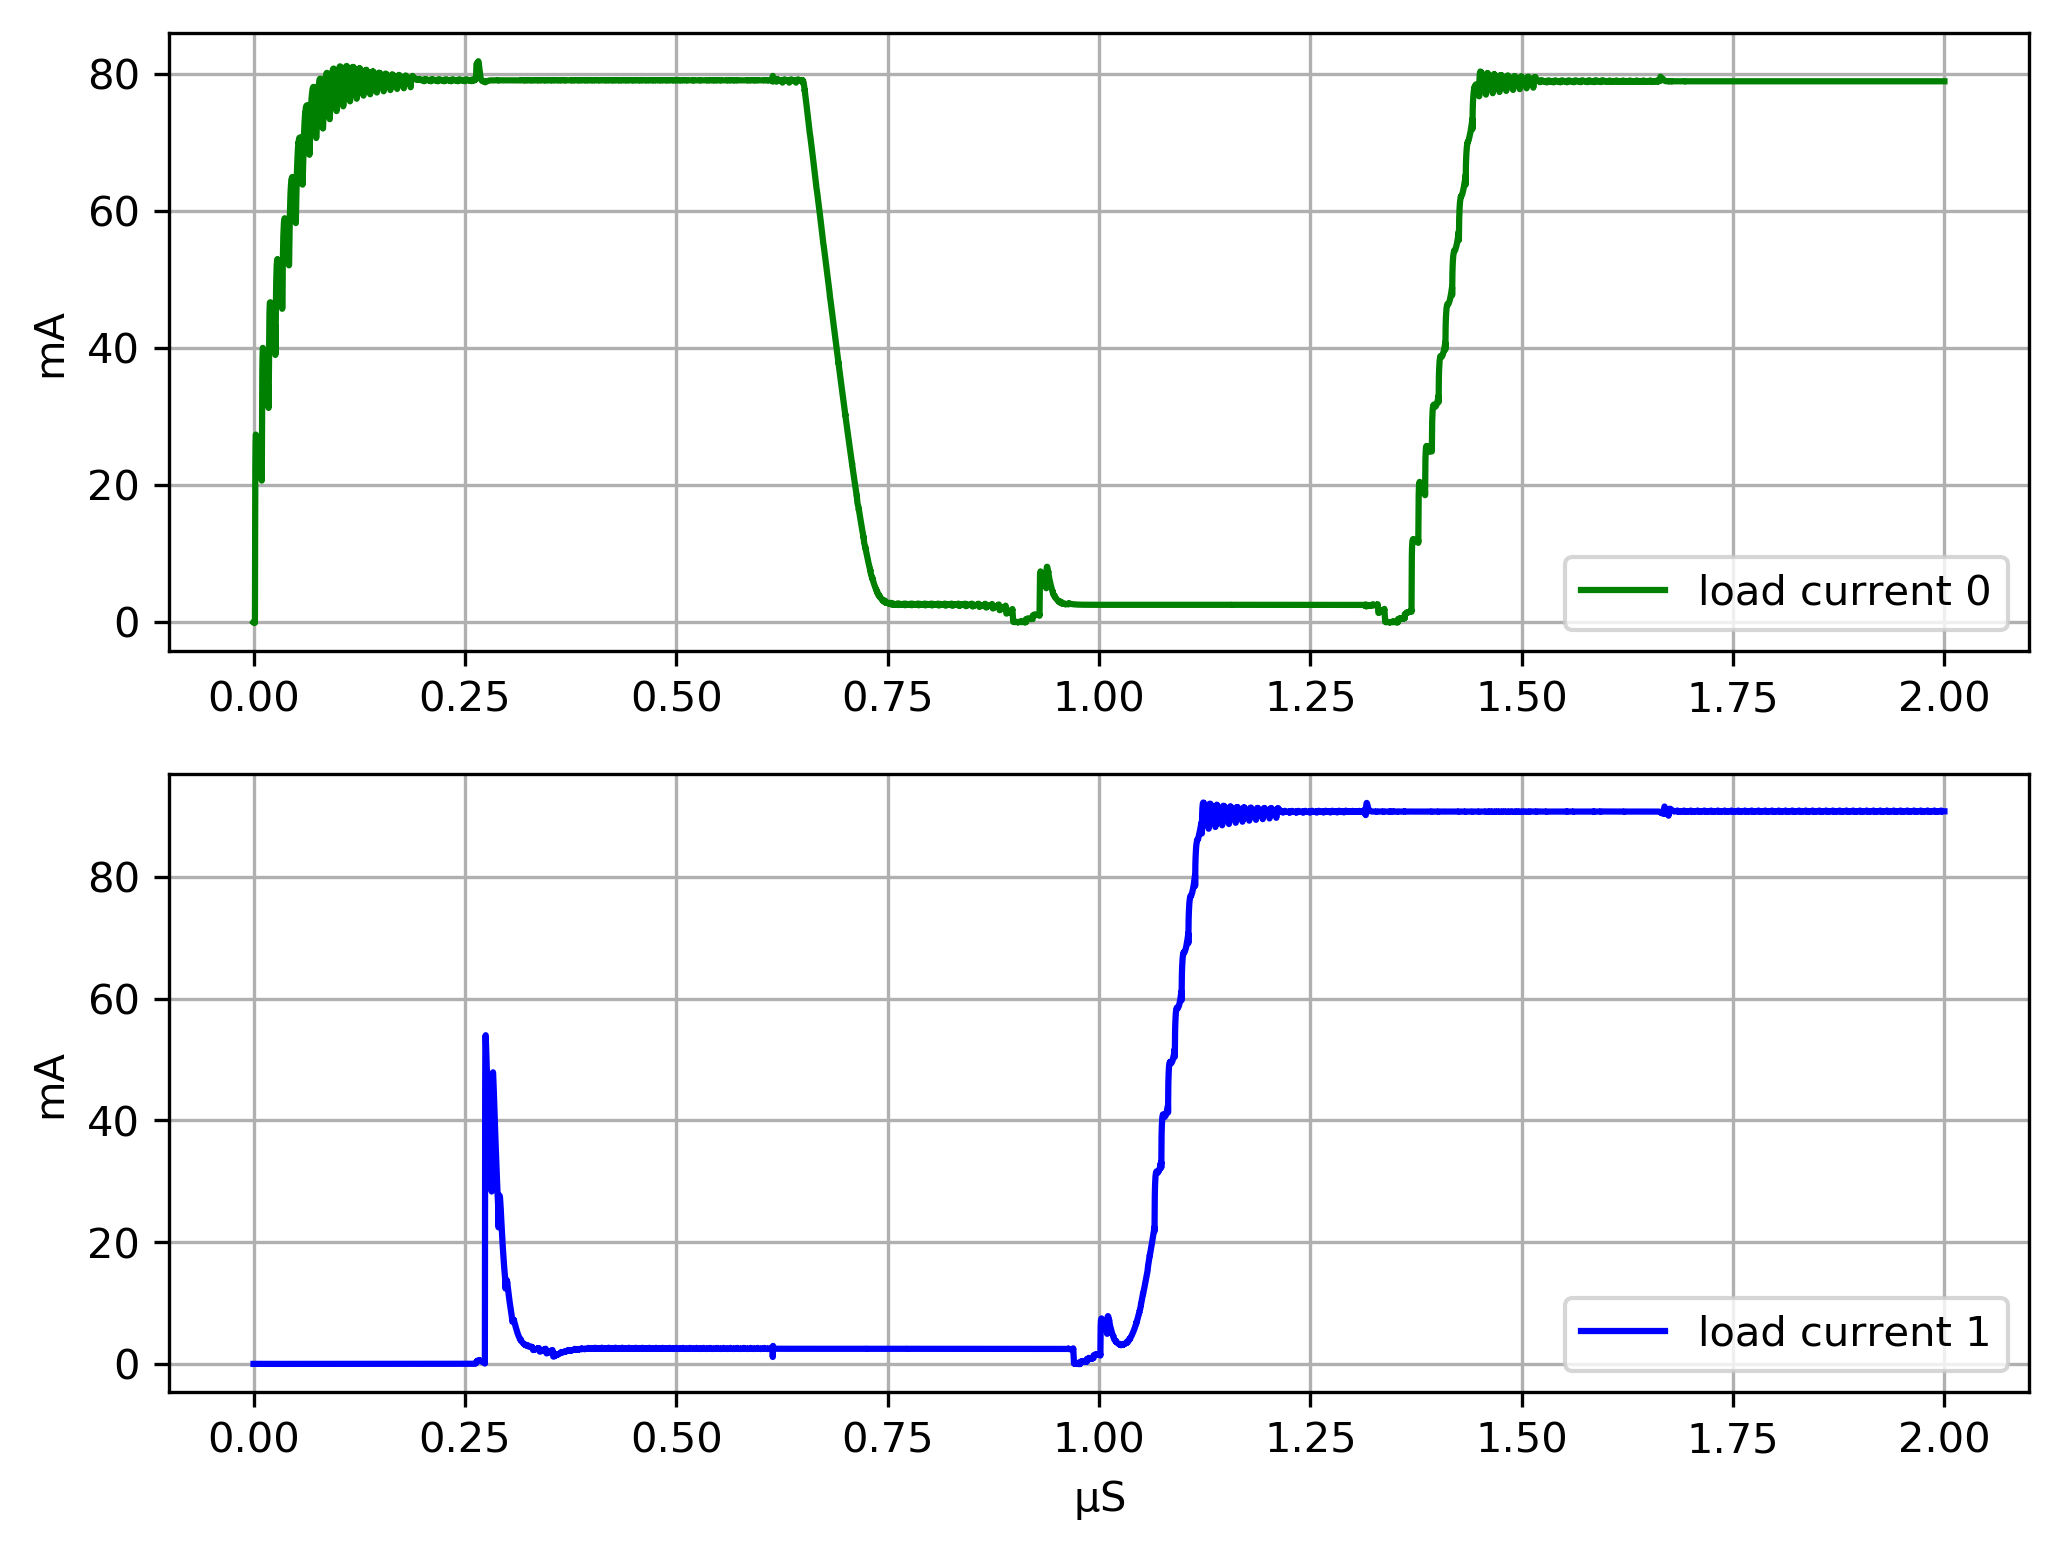
\includegraphics[width=\linewidth]{pic/resu/loadCurr.pdf}
    \caption{Load current of the two paths in TDM DLDO}
    \label{fig:curr}
\end{figure}
\begin{figure}[t!]
    \centering
    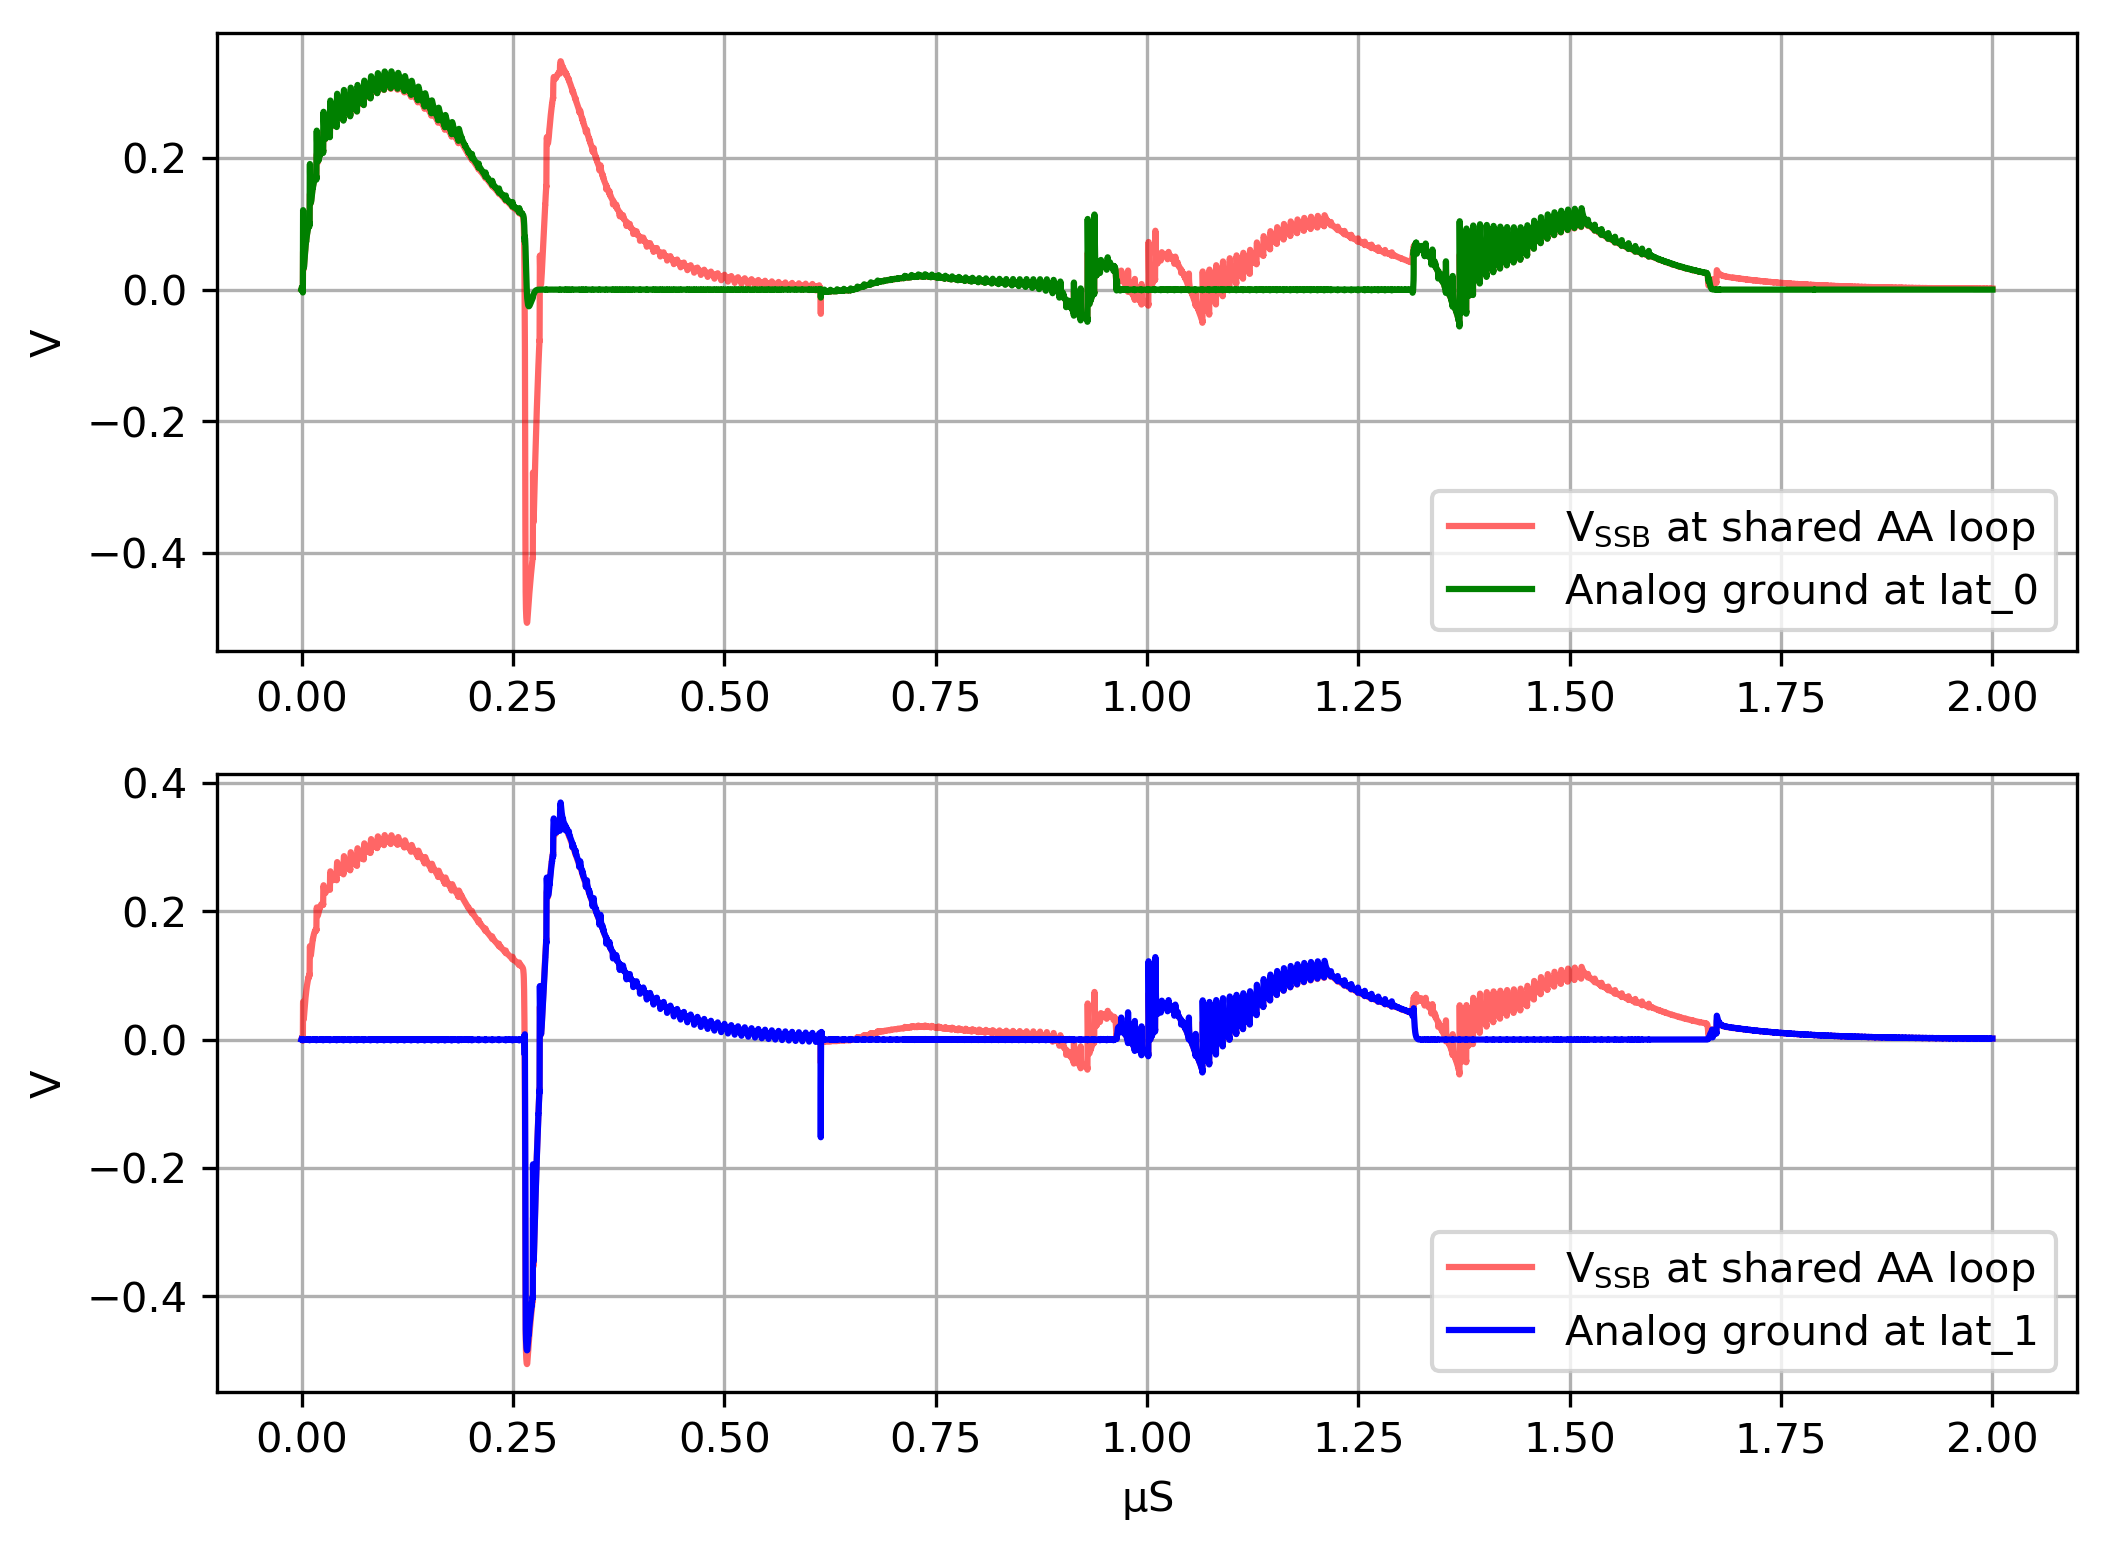
\includegraphics[width=\linewidth]{pic/resu/gnd.pdf}
    \caption{$\rm V_{SSB}$ and analog ground of latch groups}
    \label{fig:gnd}
\end{figure}
\section{Conclusion}
In this paper, we presents a novel DLDO which can share the control circuit and the shift registers between two paths. By applying the delay switching and shared AA loop techniques, we greatly reduces the total chip area and avoid the cross-channel coupling between different paths. We verify our idea through the experiment results, and it shows that the performances at two paths of the proposed TDM DLDO is comparable to the state-of-art design but chip area is greatly reduced. As the control circuit becomes more and more complicated and takes up more and more chip area, this technique provide a very promising technique to save the total chip area of the power management network. In addition, this technique can be extended to regulate more paths and reduce the total chip area even further.
\bibliographystyle{ieeetr}
\bibliography{05ref}
\end{document}


